\documentclass[11pt, oneside]{article}   	% use "amsart" instead of "article" for AMSLaTeX format
\usepackage{geometry}                		% See geometry.pdf to learn the layout options. There are lots.
\geometry{letterpaper}                   		% ... or a4paper or a5paper or ... 
%\geometry{landscape}                		% Activate for for rotated page geometry
%\usepackage[parfill]{parskip}    		% Activate to begin paragraphs with an empty line rather than an indent
\usepackage{graphicx}				% Use pdf, png, jpg, or eps§ with pdflatex; use eps in DVI mode
								% TeX will automatically convert eps --> pdf in pdflatex		
\usepackage{amssymb}
\usepackage{amsmath}
\usepackage{parskip}
\usepackage{color}
\usepackage{hyperref}

\title{Polar Cauchy-Riemann equations}
%\author{The Author}
%\section{}
%\subsection*{}
\date{}							% Activate to display a given date or no date

\graphicspath{{/Users/telliott_admin/Dropbox/Tex/png/}}
% \begin{center} 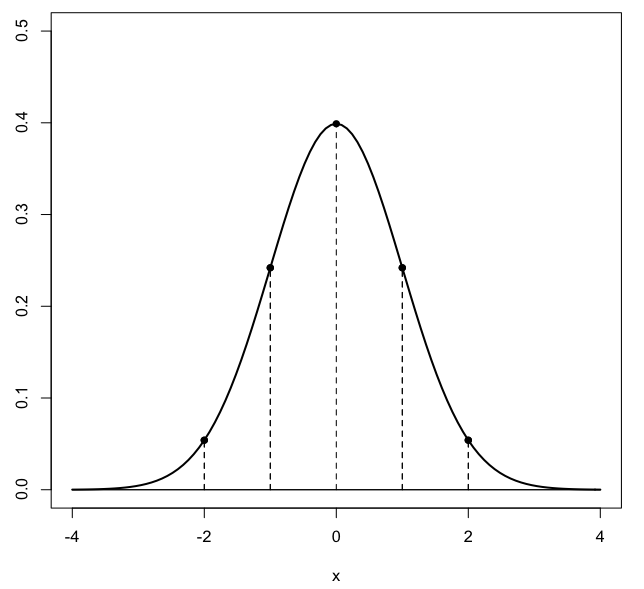
\includegraphics [scale=0.4] {gauss3.png} \end{center}
\begin{document}
\maketitle
\Large
A clever way to derive the CRE in polar coordinates is to take advantage of the result that we obtained in Cartesian coordinates.

\subsection*{short and sweet}
As we've demonstrated, the function
\[ f(z) = z = x + iy \]
is analytic, so it is differentiable.  If we write the same function in polar coordinates:
\[ z = re^{i \theta} \]
and then separate it into a completely real part $u(r, \theta)$ and a completely imaginary part $v(r,\theta)$:
\[ z = r \cos \theta + i r \sin \theta \]
Observe that $u_r = \cos \theta$ and $v_{\theta} = r \cos \theta$ so we deduce that
\[ r u_r = r \cos \theta = v_{\theta} \]
Similarly, $v_r = \sin \theta$ and $u_{\theta} = - r \sin \theta$ so we deduce that
\[ r v_r = r \sin \theta = - u_{\theta} \]
There are the CRE in polar coordinates.  Carrying out the same analysis for \emph{any} analytic function would give the same result (with some other expression in the middle, of course).

\[ r u_r = v_{\theta} \]
\[ r v_r = - u_{\theta} \]

Notice the similar format to the Cartesian version, with the addition of a factor of $r$.  Reminds me of the Jacobian from multi-variable calculus.

\subsection*{by the chain rule}

We know equations to go back and forth between $x,y$ and $r, \theta$ so it is not hard to imagine that we can always re-write $u$ and $v$ as
\[ z = u \ [ \ x(r, \theta), y(r, \theta) \ ] + i v \ [ \ x(r,\theta),y(r, \theta) \ ] \]
or more succinctly:
\[ z = u(r, \theta) + i v(r, \theta) \]

Now we ask about relations between the partial derivatives.

Obviously, we want expressions involving $u_r$, $v_{\theta}$ etc.  Write:
\[ \frac{\partial u}{\partial r} = \frac{\partial u}{\partial x} \frac{\partial x}{\partial r} + \frac{\partial u}{\partial y} \frac{\partial y}{\partial r} \]

or using the convenient shorthand
\[ u_r = u_x x_r + u_y y_r \]

Now, we know
\[ x = r \cos \theta \]
\[ y = r \sin \theta \]
and the derivatives are
\[ x_r = \cos \theta \]
\[ x_{\theta} = -r \sin \theta \]
\[ y_r = \sin \theta \]
\[ y_{\theta} = r \cos \theta \]

Now write the four expansions (like the one given above) as:
\[ u_r = u_x x_r + u_y y_r = u_x \cos \theta + u_y \sin \theta \]
\[ v_r = v_x x_r + v_y y_r = v_x \cos \theta + v_y \sin \theta \]
\[ u_{\theta} = u_x x_{\theta} + u_y y_{\theta} = u_x (-r \sin \theta) + u_y (r \cos \theta) \]
\[ v_{\theta} = v_x x_{\theta} + v_y y_{\theta} = v_x (-r \sin \theta) + v_y (r \cos \theta) \]

Our key insight is to substitute the relations given by the CRE in Cartesian coordinates ($u_x = v_y$, $u_y = - v_x$).  In the first above we get
\[ u_r = u_x \cos \theta + u_y \sin \theta = v_y \cos \theta - v_x \sin \theta = \frac{1}{r} v_{\theta} \]
(where the final step equating to $v_{\theta}/r$ uses the last equation).

In the second
\[ v_r = v_x \cos \theta + v_y \sin \theta = -u_y \cos \theta + u_x \sin \theta = - \frac{1}{r} u_{\theta} \]
(and the last step uses the third equation).

In other words:
\[ r u_r = v_{\theta} \]
\[ r v_r = - u_{\theta} \]
which is what needed to prove.

Like the original Cartesian version but with an extra factor of $r$.

\section*{polar derivative} 
This will also turn out to be very similar to the Cartesian version, with a twist, which is that we have an extra factor out front:
\[ f'(z) = e^{-i \theta} \ [ \ u_r + i v_r \ ] \]

\subsection*{short and sweet}
Let's just assume that the derivative is equal to what we would expect, within some unknown factor of $k$:
\[ z' = k(u_r + i v_r) \]
and now we know that for this function the derivative is equal to $1$:
\[ f(z) = z \]
\[ z' = 1 = k(u_r + i v_r) \]
if we write in polar coordinates:
\[ z = r \cos \theta + i r \sin \theta \]
Then 
\[ u_r + i v_r = \cos \theta + i \sin \theta \]
What is the factor that multiplies this expression to give $1$?
Clearly
\[ e^{- i \theta} (\cos \theta + i \sin \theta) = 1 \]
So $k = e^{- i \theta}$.

\subsection*{more carefully}

To get the derivative, start with the version that we know for $x,y$ coordinates:
\[ f'(z) = u_x + i v_x \]

Our problem is to define $f'(z)$ in terms of $u_r$ and $v_r$.

Substitute for $u_x$ first.  Go back to the two equations involving $u_x$ above
\[ u_r = u_x \cos \theta + u_y \sin \theta \]
\[ u_{\theta} = u_x (-r \sin \theta) + u_y (r \cos \theta) \]

Multiply the first by $\cos \theta$
\[ u_r \cos \theta = u_x \cos^2 \theta + u_y \sin \theta \cos \theta \]
 and the second by $- \sin \theta/r$
\[ - \frac{u_{\theta}}{r} \sin \theta = u_x  \sin^2 \theta - u_y \sin \theta \cos \theta \]
add
\[ u_x = u_r \cos \theta - \frac{u_{\theta}}{r} \sin \theta \]
Substitute $u_{\theta}/r = - v_r$
\[ u_x = u_r \cos \theta + v_r \sin \theta \]

Now get the second and fourth equations, with $v_x$
\[ v_r = v_x \cos \theta + v_y \sin \theta \]
\[ v_{\theta} = v_x (-r \sin \theta) + v_y (r \cos \theta) \]

Multiply the first by $\cos \theta$
\[ v_r \cos \theta = v_x \cos^2 \theta + v_y \sin \theta \cos \theta \]
and the second by $-\sin \theta / r$:
\[ -\frac{v_{\theta}}{r} \sin \theta = v_x \sin^2 \theta - v_y \sin \theta \cos \theta \]
add
\[ v_x = v_r \cos \theta -\frac{v_{\theta}}{r} \sin \theta \]
Subtitute $v_{\theta}/r = u_r$
\[ v_x = v_r \cos \theta - u_r \sin \theta \]

Combine the two results:
\[ f'(z) = u_x + i v_x \]
\[ = u_r \cos \theta + v_r \sin \theta + i \ [ \ v_r \cos \theta - u_r \sin \theta \ ] \]
Group terms with $u_r$ and $v_r$ separately:
\[ = u_r (\cos \theta - i \sin \theta) + v_r (\sin \theta + i \cos \theta)  \]
Multiply the second term by $1 = - i \cdot i$
\[ = u_r (\cos \theta - i \sin \theta) + i v_r (- i \sin \theta + \cos \theta)  \]
\[ f'(z) = e^{-i \theta} \ [ \ u_r + i v_r \ ] \]

And since
\[ r u_r = v_{\theta} \]
\[ r v_r = -u_{\theta} \]
then
\[ f'(z) = \frac{1}{r} \ e^{-i \theta} \ [ \ v_{\theta} - i u_{\theta} \ ] \]
compare this with 
\[ f'(z) = v_y - iu_y \]
and notice that the factor in front is just $1/z$

\subsection*{example 1}

Let's see if we can do an example.  Suppose
\[ f(z) = \sqrt{z} \]
Written in terms of $r, \theta$ we have
\[ f(z) = \sqrt{r} e^{i \theta/2} \]
\[ = \sqrt{r} \cos \theta/2 + i \sqrt{r} \sin \theta/2 \]
Then
\[ u_r = \frac{\cos \theta/2}{2 \sqrt{r}} \]
\[ v_r = \frac{\sin \theta/2}{2 \sqrt{r}} \]
and
\[ \ [ \sqrt{z} \ ]' = \ [ \ \sqrt{r} e^{i \theta/2} \ ]' = e^{-i \theta} \ [ \ u_r + i v_r \ ] \]
\[ = \frac{1}{2 \sqrt{r}} \ [ \ e^{-i \theta} (\cos \theta/2 + i \sin \theta/2) \ ]    \]
\[ = \frac{1}{2 \sqrt{r}} e^{-i \theta/2} = \frac{1}{2 \sqrt{z}} \]

\subsection*{example 2}
Let's try
\[ f(z) = \frac{1}{z} = \frac{1}{r} e^{-i \theta} \]
\[ = \frac{1}{r} \cos - \theta + i \frac{1}{r} \sin - \theta \]
\[ = \frac{1}{r} \cos \theta - i \frac{1}{r} \sin \theta \]
So
\[ u_r = -\frac{1}{r^2} \cos \theta \]
\[ v_r = \frac{1}{r^2} \sin \theta \]
\[ f'(z) = e^{-i \theta}  (u_r + i v_r) \]
\[ \frac{1}{r^2} ( e^{-i \theta}) (- \cos \theta + i \sin \theta) \]
\[ \frac{1}{r^2} ( e^{-i \theta}) (- \cos - \theta - i \sin - \theta) \]
\[ \frac{1}{r^2} ( e^{-i \theta}) (-1) (e^{-i \theta}) \]
\[ = -\frac{1}{r^2 e^{i 2\theta}} = -\frac{1}{z^2} \]

\end{document} 